\documentclass[tikz,border=3.14mm]{standalone}
\begin{document}
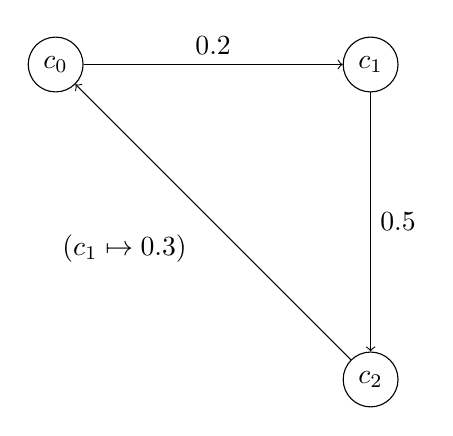
\begin{tikzpicture}
    \node[circle,draw] (c0) at (0,4) {$c_0$};
    \node[circle,draw] (c1) at (4,4) {$c_1$};
    \node[circle,draw] (c2) at (4,0) {$c_2$};

    \draw[->] (c0) -- node[above] {0.2} (c1);
    \draw[->] (c1) -- node[right] {0.5} (c2);
    \draw[->] (c2) -- node[below left] {\begin{tabular}{c}$(c_1 \mapsto 0.3)$\\ \end{tabular}} (c0);
\end{tikzpicture}
\end{document}